\section[Usage]{Usage statistics and uptake}
\label{variantcalling-sec:usage}
\remove{Ultimately}When choosing research software, publication and citations are not \remove{a} good metric\add{s} to evaluate the quality of a method \cite{Gardner2022}. Many published software packages are not maintained or not even functional even though they are published. While we developed these joint somatic variant calling workflows to deal with a challenge we faced, the interest of others has been continuously expressed by other members of the bioinformatics community  in the \remove{short period of} time since publication.

\begin{figure}[!ht]
\centering
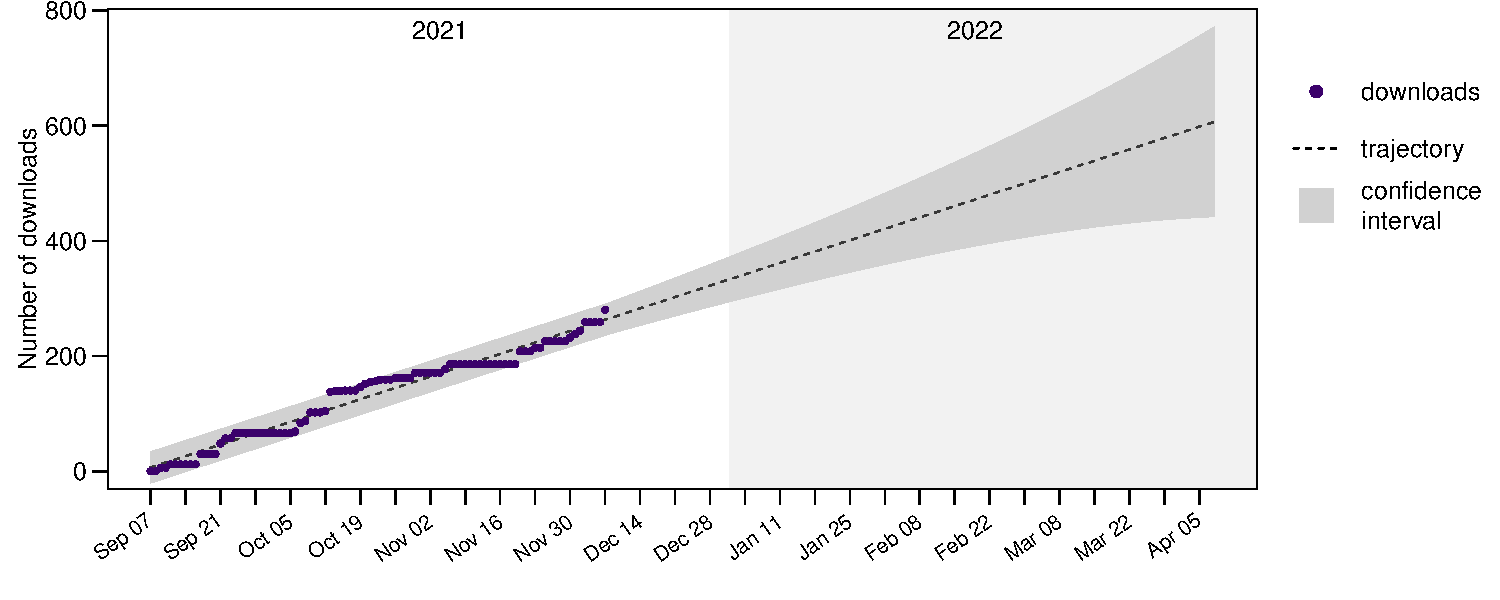
\includegraphics[width=.99\linewidth]{Figures/jointVariantCalling/dawsontoolkitDownloads.pdf}
\caption[Usage statistics joint workflows]{Cumulative download numbers of the ``dawsontoolkit`` docker container since publication of the manuscript; Actual counts are shown as dots, with smoothed trajectory depicted as dotted line with the 95\% confidence interval shown as a grey background; confidence interval has been adjusted with exponential decay of prediction accuracy with distance from the last data point; Start date 7$^{th}$ September 2021 (publication of method); End point prediction 31$^{th}$ December 2022 (End of current year); Numbers were recorded daily from the DockerHub API}\label{fig:usageStats}
\end{figure}

To have some proxy of the usage statistics of the workflows, we recorded the download numbers of the ``dawsontoolkit`` docker container after the publication of the manuscript. The container only consists of software for refiltering and joint analysis of the workflows. \remove{Obviously, }This is an imperfect measurement, as people can reuse a downloaded container as often as they want, which would not appear in the count and similarly, just because the container was downloaded, the analysis might not have been used. Nevertheless, it still shows \remove{an} interaction and \remove{an} interest in the methods. The download numbers show a sustained and stable increase in downloads (\autoref{fig:usageStats}). These numbers suggest that there is a need \change{in}{for} the methods rather than a simple curiosity after publication, which, hopefully, will facilitate a higher quality analysis of future projects and \remove{therefore} lead to a better understanding of cancer evolution and heterogeneity.
